

\subsection{Two Dimensional Delaunay}
\label{sec:delaunay_2_example}

As with static triangulations, in order to use the data structure the
user must provide a traits class. In addition, an optional visitor
class can be provided to monitor how the data structure changes, and a
custom triangulation can be provided. The traits class must be a model
of \ccc{SimulationTraits}. Most of the details of the traits class can
be ignored for the time being other than two parts 
\begin{description}
\item[\ccc{moving_point_table_pointer()}] this returns a (reference counted) pointer to a table which keeps track of all the primitives.
\item[\ccc{simulator_pointer()}] this returns a pointer to the \ccc{Simulator} which is what controls how time advances.
\end{description}
The framework provides a number of models of the
\ccc{SimulationTraits} named
\{Exact,Inexact\}\_simulation\_traits\_\{1,2,3\}. Here we opt for
exact computations (and require two dimensions).

In order to monitor the Delaunay triangulation as the simulation is
run, we use a visitor. This is a small class, which is passed to the
Delaunay triangulation. The triangulation calls methods on the visitor
class whenever things happen. In the case, the visitor,
\ccc{CGAL::KDS::Delaunay_triangulation_event_log_visitor_2} simply makes a record of each event that occurs.

Once the traits class and kinetic Delaunay have been created, we need4
to add points to the simulation. To do this, we add them directly to
the
\ccc{ActiveObjectsTable} using the \ccc{insert} method. 


Now that the triangulation has been set up at points added (or
scheduled for addition), we can run the kinetic data structure. Here
we ask the simulation to process all events and then using the visitor
to print out a record of all events that occur. Note that there are a
finite number of events since eventually all the points are spead far
apart and simply moving outward. If instead, we had added a
\ccc{CGAL::KDS::Enclosing_box_2<Traits>} to the simulation, then 
there would be an infinite number of events as the points repeatedly
bounce off the walls.

For an equivalent example with a graphical interface, see
demo/Kinetic\_data\_structures/Delaunay\_triangulation\_2.C.

\begin{figure*}[htb]
\begin{ccTexOnly}
\begin{center}
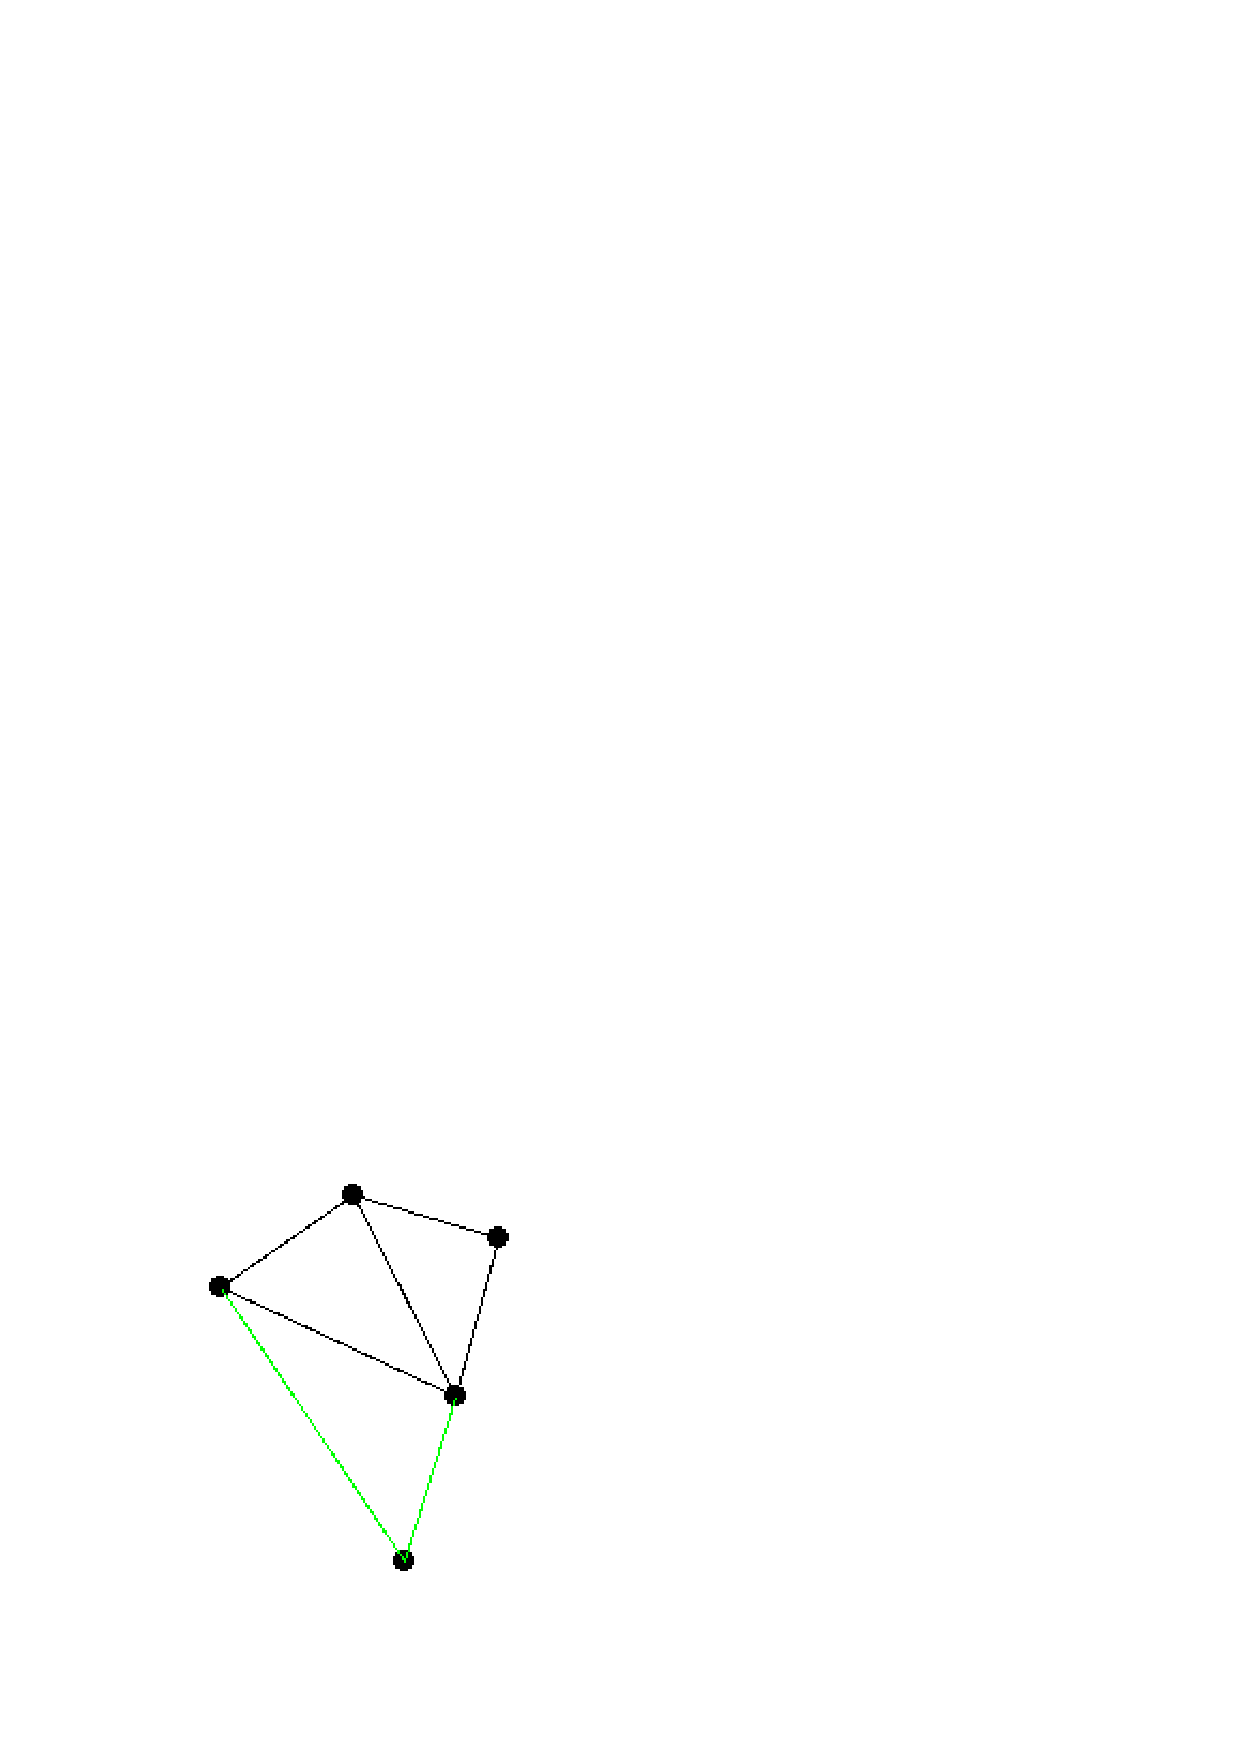
\includegraphics[ scale=.3]{Kinetic_data_structures/delaunay_shot_0_crop_pct} 
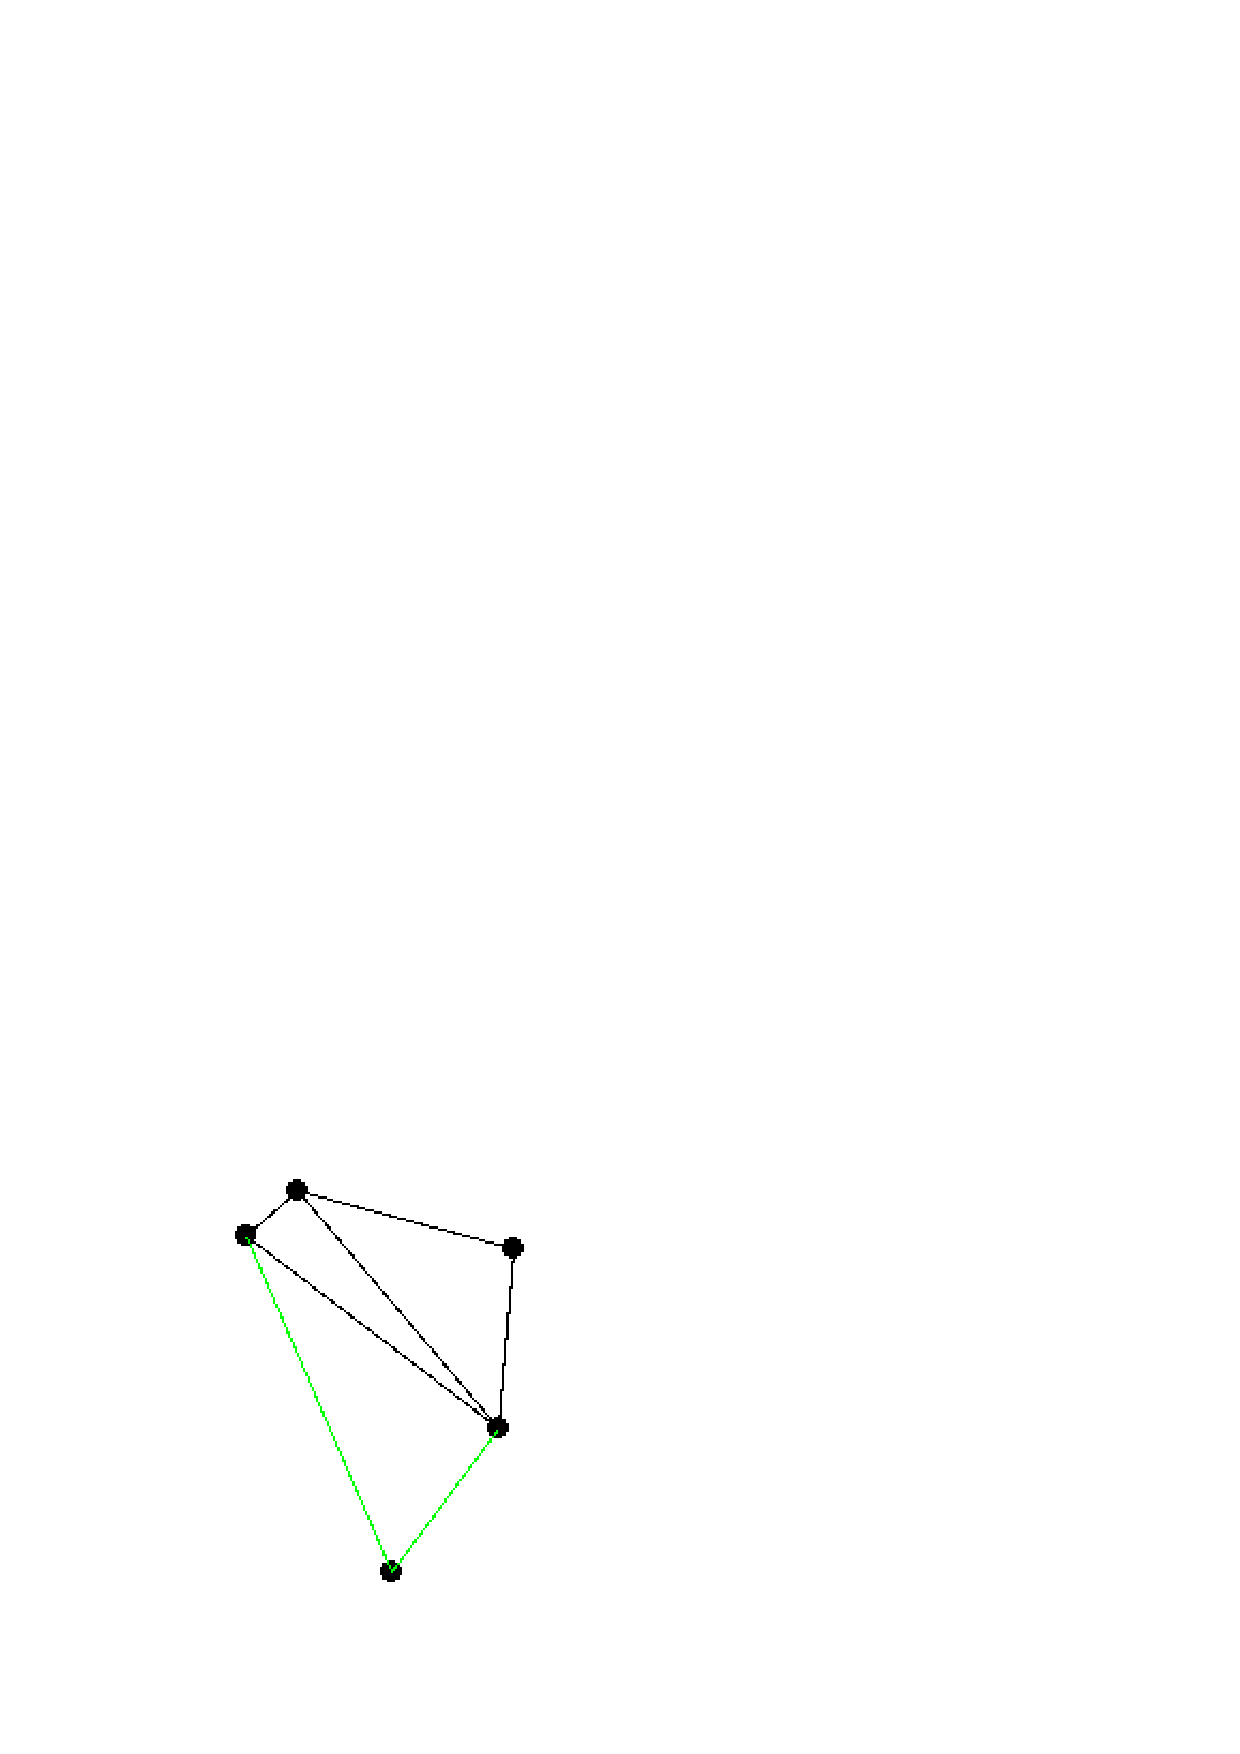
\includegraphics[ scale=.3]{Kinetic_data_structures/delaunay_shot_1_crop_pct}
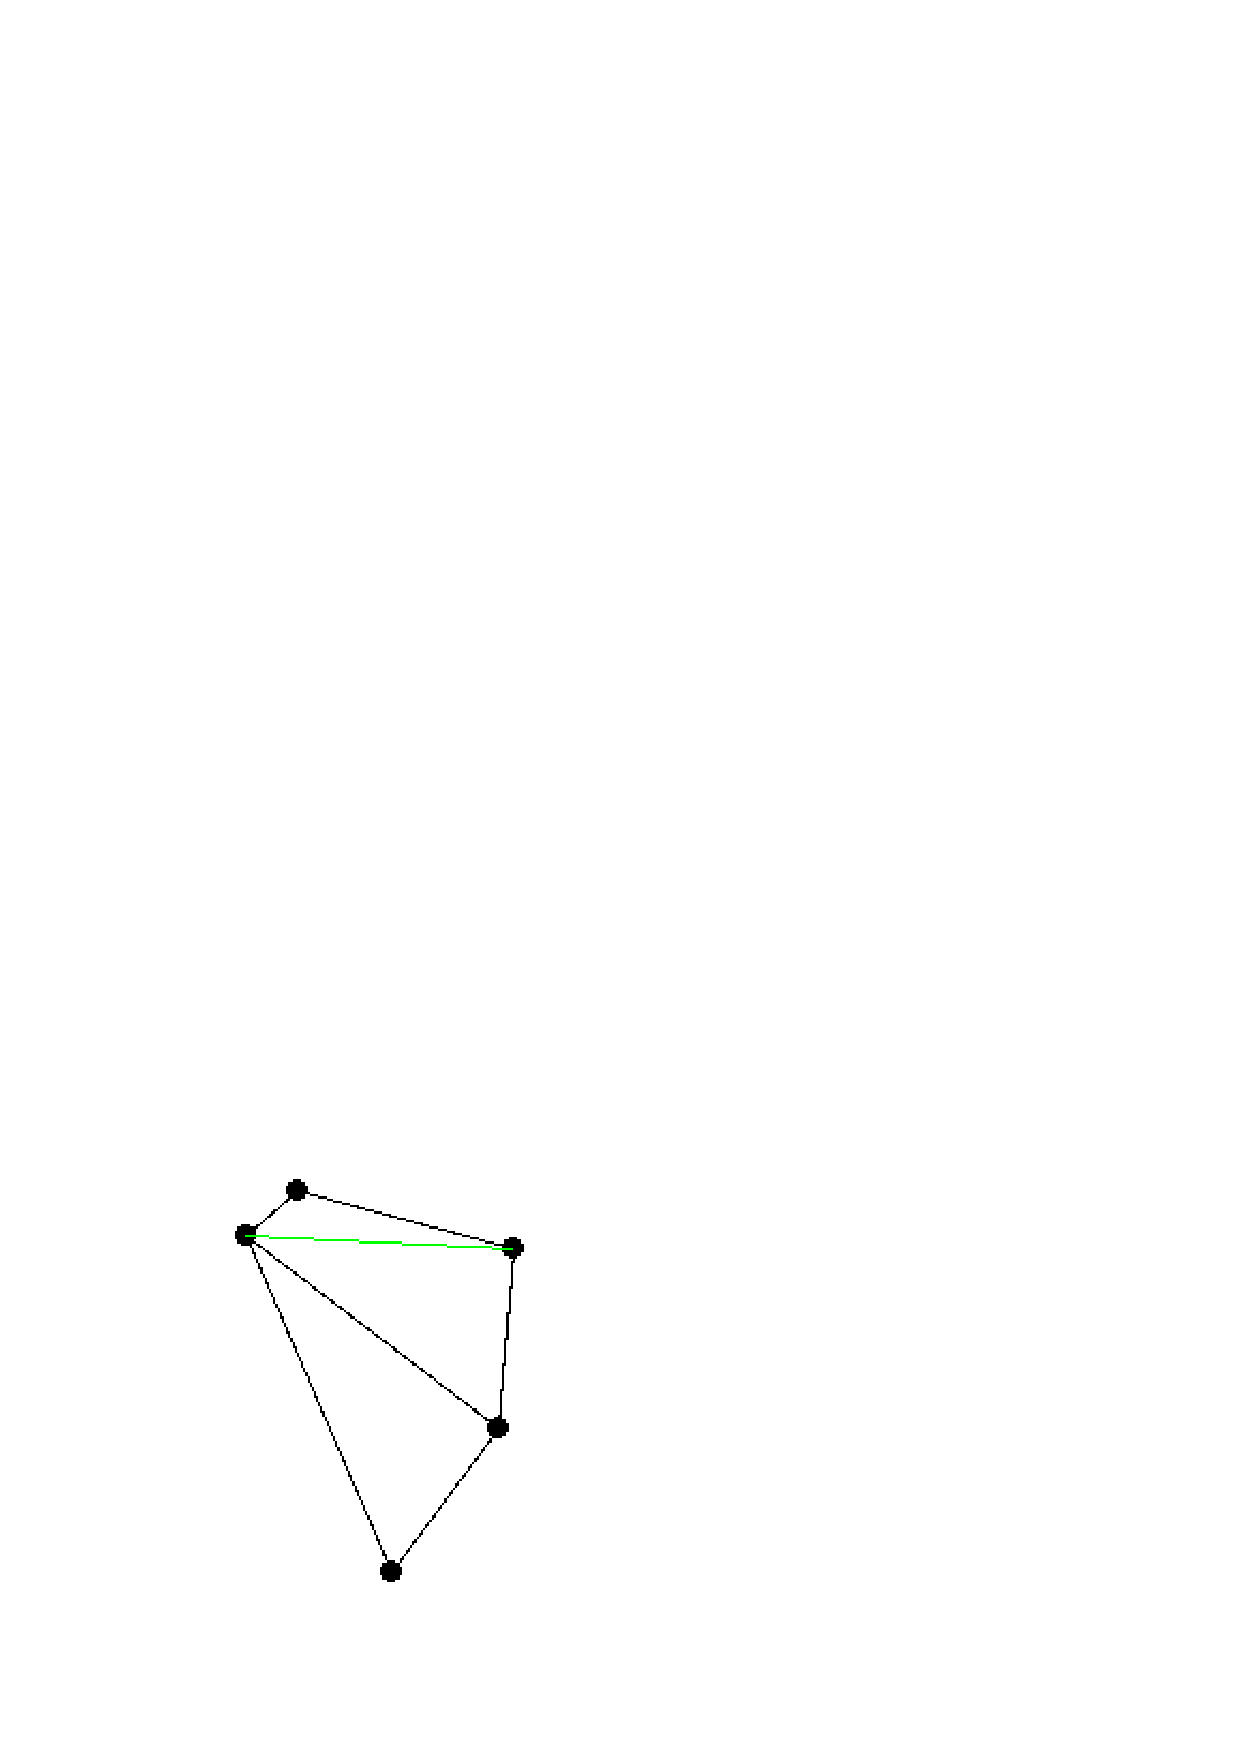
\includegraphics[ scale=.3]{Kinetic_data_structures/delaunay_shot_2_crop_pct}
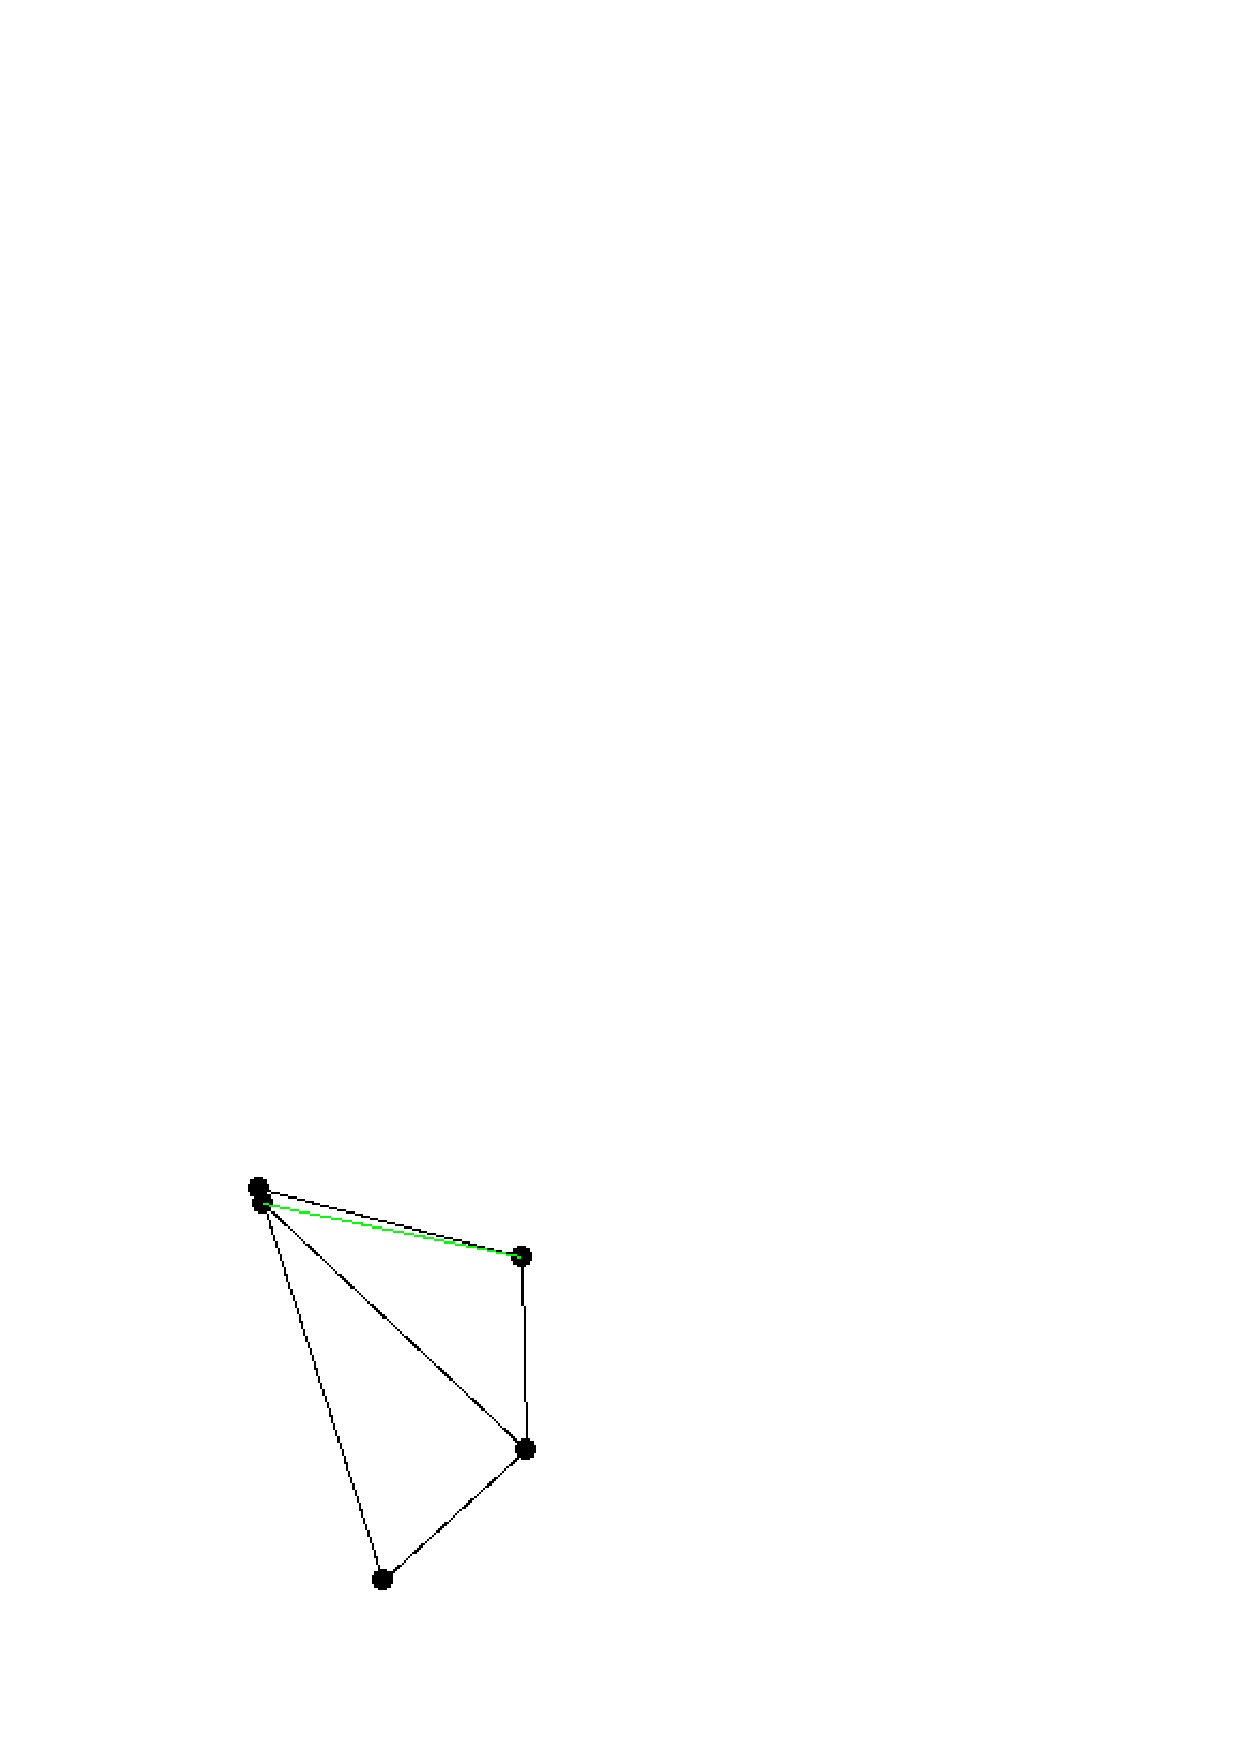
\includegraphics[ scale=.3]{Kinetic_data_structures/delaunay_shot_3_crop_pct}\\
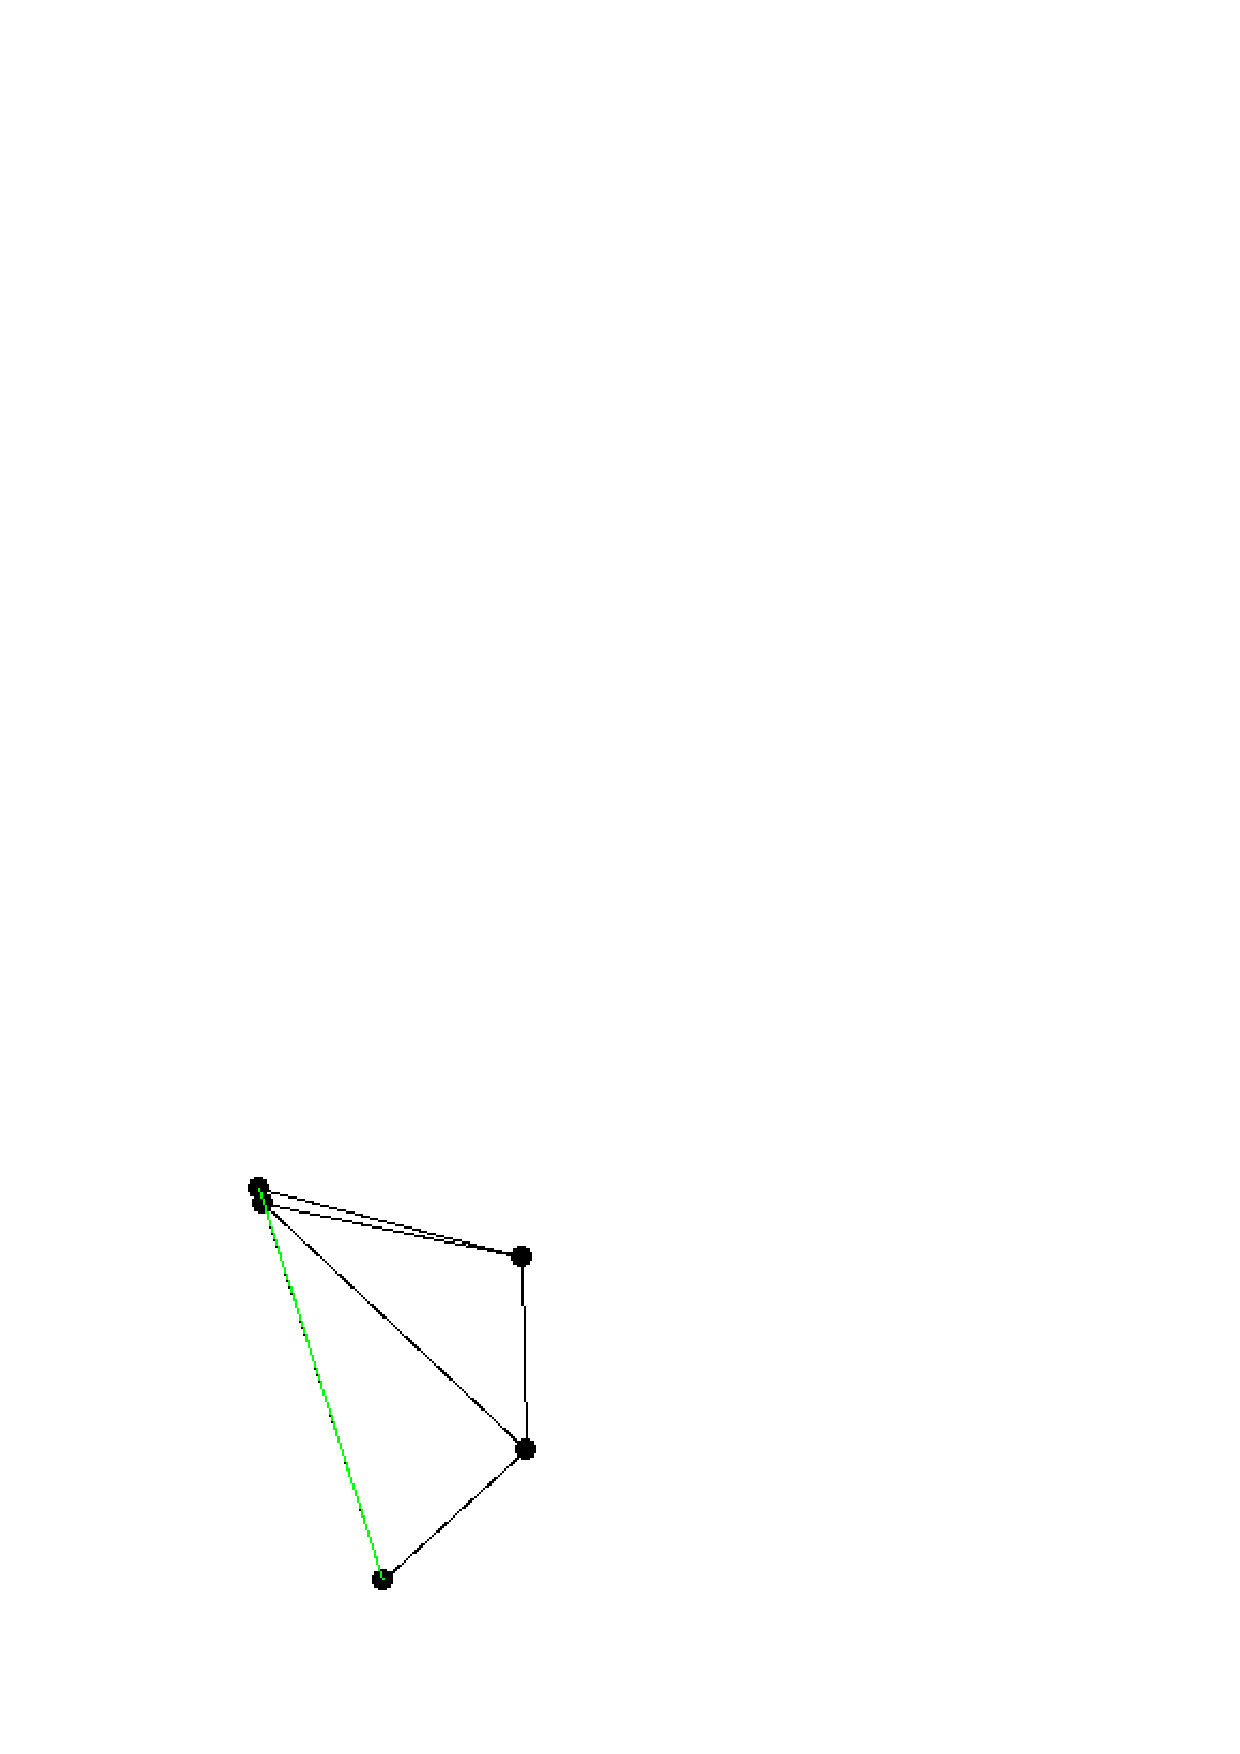
\includegraphics[ scale=.3]{Kinetic_data_structures/delaunay_shot_4_crop_pct}
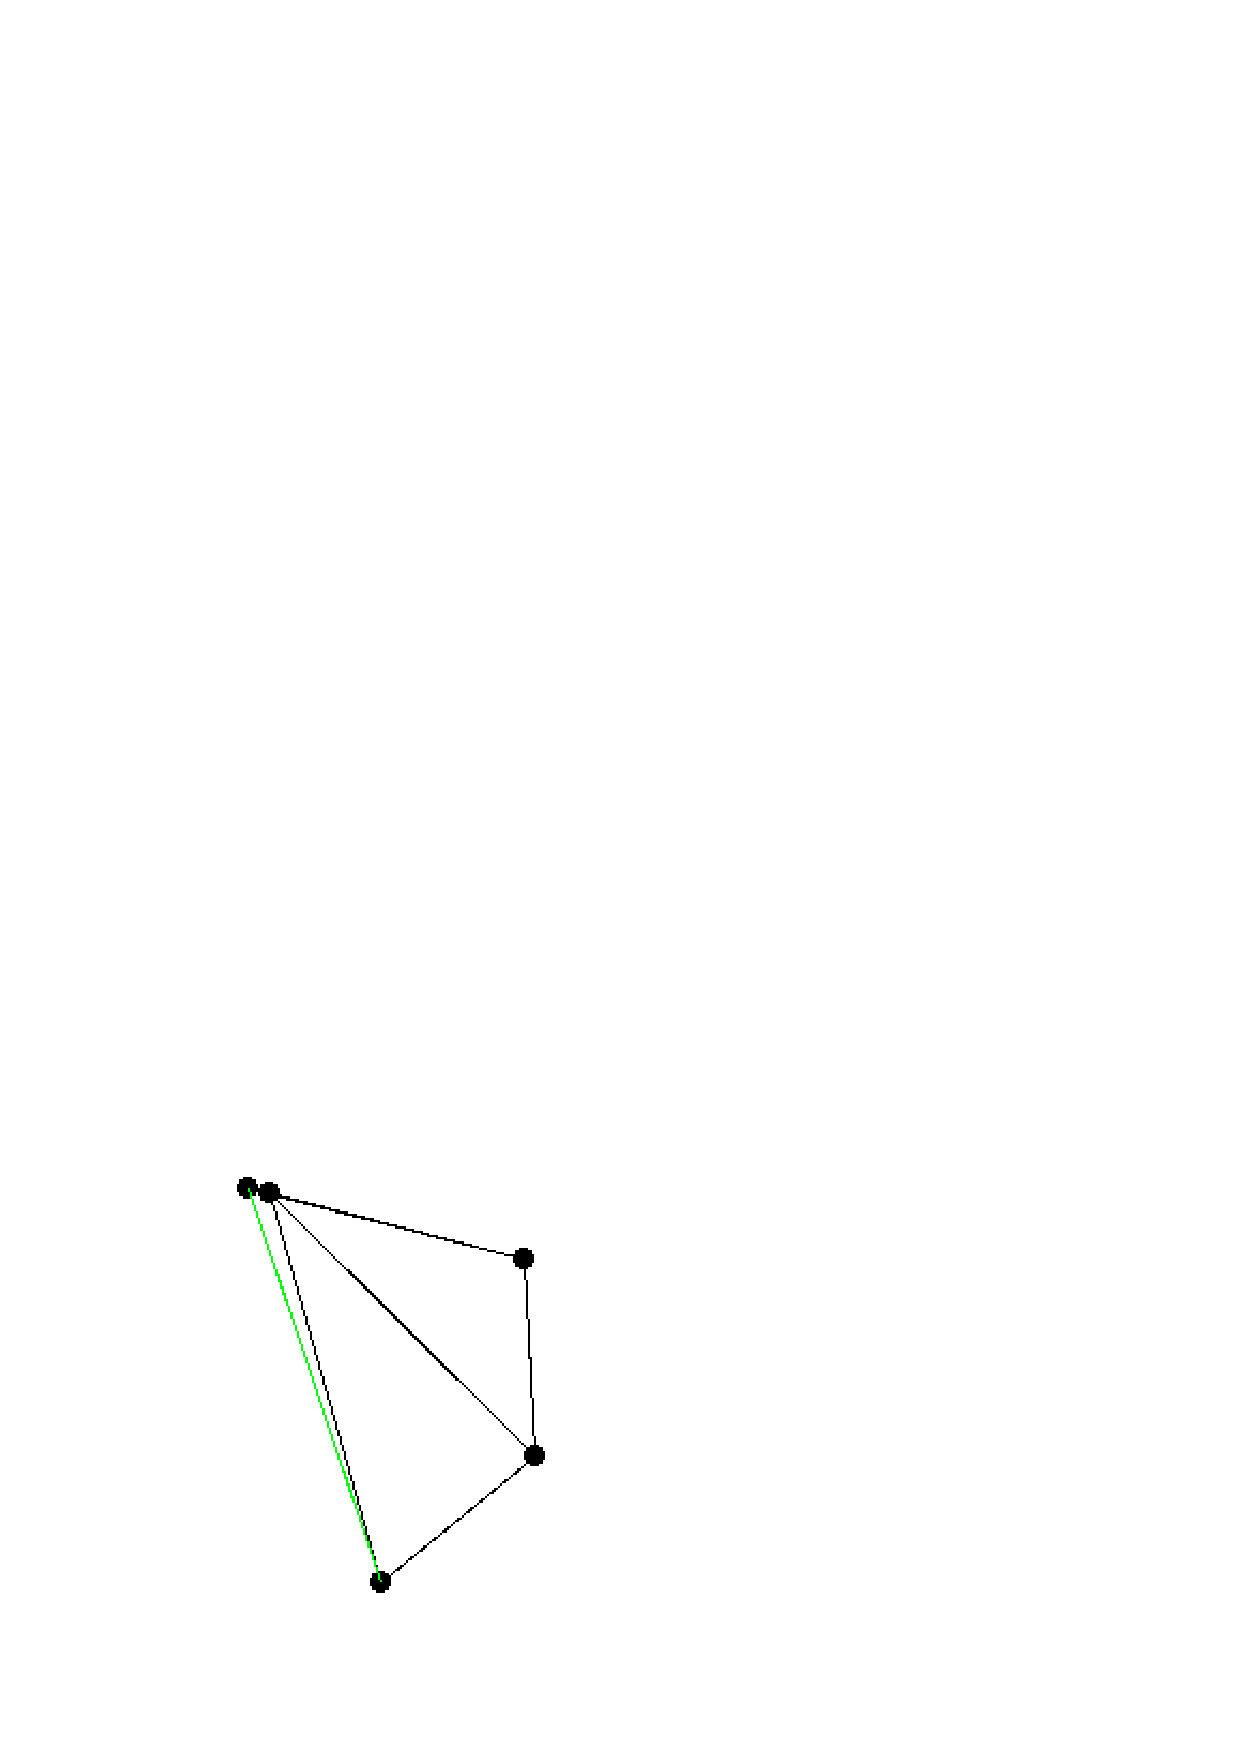
\includegraphics[ scale=.3]{Kinetic_data_structures/delaunay_shot_5_crop_pct}
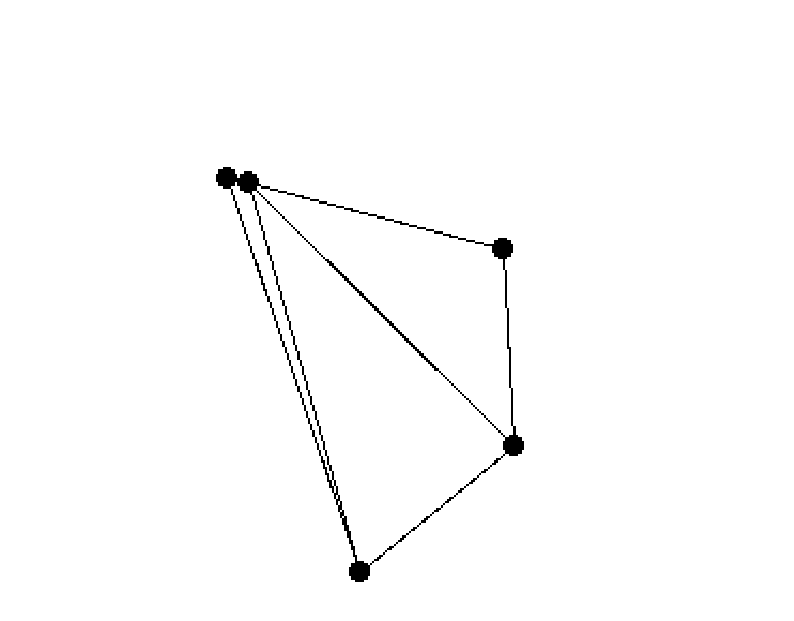
\includegraphics[ scale=.3]{Kinetic_data_structures/delaunay_shot_6_crop_pct}
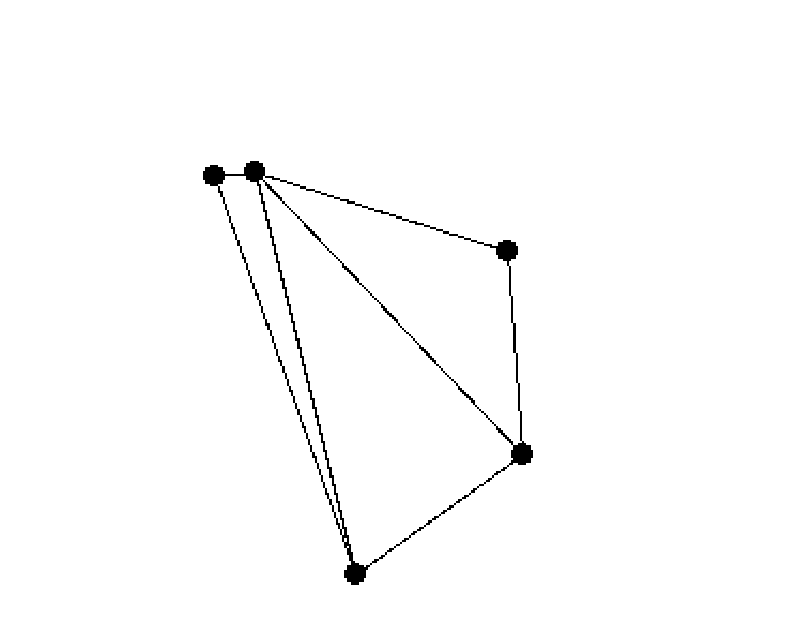
\includegraphics[ scale=.3]{Kinetic_data_structures/delaunay_shot_7_crop_pct}\\
\end{center}
\end{ccTexOnly}
\begin{ccHtmlOnly}
<center>
<imp border=1 src="Kinetic_data_structures/delaunay_shot_0.crop.png" align=center alt="Frame 0">
<imp border=1 src="Kinetic_data_structures/ddelaunay_shot_1.crop.png" align=center alt="Frame 1">
<imp border=1 src="Kinetic_data_structures/ddelaunay_shot_2.crop.png" align=center alt="Frame 2">
<imp border=1 src="Kinetic_data_structures/ddelaunay_shot_3.crop.png" align=center alt="Frame 3">
<imp border=1 src="Kinetic_data_structures/ddelaunay_shot_4.crop.png" align=center alt="Frame 4">
<imp border=1 src="Kinetic_data_structures/ddelaunay_shot_5.crop.png" align=center alt="Frame 5">
<imp border=1 src="Kinetic_data_structures/ddelaunay_shot_6.crop.png" align=center alt="Frame 6">
<imp border=1 src="Kinetic_data_structures/ddelaunay_shot_7.crop.png" align=center alt="Frame 7">
</center>
\end{ccHtmlOnly}
\caption{ \label{fig:delaunay_events} 
{\em Some events from a Delaunay triangulation kinetic data structure:} Before and after the first several events in a kinetic data structure is shown. The pictures are screen shots from demo/Kinetic\_data\_structures/Delaunay\_triangulation\_2.C. }
%\end{minipage}
%\end{center}
\end{figure*}


\label{fig:delaunay_2_usage_program}
\ccIncludeExampleCode{Kinetic_data_structures/Delaunay_triangulation_2.C}
